\documentclass[11pt,a4paper]{article}
\usepackage[margin=1in]{geometry}
\usepackage{amsmath,amssymb,amsfonts}
\usepackage{graphicx}
\usepackage{booktabs}
\usepackage{hyperref}

\title{\textbf{Functionally Graded Dual-Scale Horizon Blending and Moment-Corrected Stiffness for Ghost-Force-Free and Reflection-Free Multiscale Peridynamics}}
\author{Mohamadreza Soltani \\ \small Native macOS Apple Silicon (\texttt{arm64}) SALOME Peridynamics Framework}
\date{\today}

\begin{document}
\maketitle

\begin{abstract}
Coupling fine and coarse spatial discretizations in variable-horizon Bond-Based Peridynamics (BB-PD) introduces two distinct numerical artifacts at resolution interfaces: (i) static \emph{ghost forces} under uniform strain caused by broken bond-horizon symmetry, and (ii) dynamic \emph{spurious wave reflections} caused by abrupt jumps in the nonlocal dispersion relation $\omega(k,\delta)$. In this work, we demonstrate mathematically and numerically that grading the horizon $\delta(x) = m\Delta x(x)$ like a Functionally Graded Material (FGM) without stiffness correction spreads the ghost force across the transition zone rather than eliminating it. However, by combining (1) a $C^1$ Functionally Graded Dual-Scale Horizon Blending law in the transition zone with (2) a symmetric energy-consistent and third-order moment-projected stiffness correction $g_{ij}$, we achieve exact linear momentum conservation ($\|\sum_i \mathbf{F}_i\| \sim 10^{-17}$), machine-precision zero ghost forces ($\|\mathbf{f}_{\mathrm{ghost}}\|_{\infty} < 10^{-12}$) across 1D, 2D, and 3D graded meshes, and a reduction in spurious wave reflection from $7.73\%$ (uncorrected) and $0.22\%$ (abrupt ghost-free) down to $0.030\%$ ($99.97\%$ clean wave transmission).
\end{abstract}

\section{Introduction}
Peridynamics reformulates continuum mechanics via nonlocal integral equations over a finite horizon $\delta_i = m\Delta x_i$. To resolve localized crack tips efficiently in 3D engineering components exported from SALOME (\texttt{.med} and \texttt{.unv}), $\Delta x_i = V_i^{1/d}$ must transition from fine spacing $\Delta x_f$ near defects to coarse spacing $\Delta x_c$ in the far field.

Existing variable-horizon formulations face a fundamental trade-off between static equilibrium and dynamic wave transmission. As shown in Fig.~1 and Fig.~2, interface errors arise from two physically distinct sources:
\begin{enumerate}
  \item \textbf{Static Ghost Force:} Under uniform strain $\mathbf{u}(\mathbf{x}) = \boldsymbol{\varepsilon}\mathbf{x}$, any spatial gradient $\nabla \delta(\mathbf{x}) \neq \mathbf{0}$ breaks the odd-order directional moments of the micromodulus.
  \item \textbf{Dynamic Dispersion Reflection:} Even when static ghost forces vanish, the nonlocal dispersion relation $\omega^2(k,\delta) = \frac{2E}{\rho\delta^2}\int_0^{\delta}(1-\cos k\xi)\,d\xi$ yields different group velocities on fine and coarse grids, causing short-wavelength wave packets to reflect at sharp interfaces.
\end{enumerate}

\section{Functionally Graded Dual-Scale Horizon Formulation}
Across a transition zone $x \in [x_a, x_b]$ of width $L_{\mathrm{FGM}}$, we define a $C^1$-continuous cosine volume-fraction law:
\begin{equation}
  w(\xi) = \frac{1}{2}\bigl(1 - \cos(\pi\xi)\bigr), \qquad \xi = \mathrm{clip}\!\left(\frac{x - x_a}{L_{\mathrm{FGM}}}, 0, 1\right), \qquad \Delta x(x) = (1 - w(\xi))\Delta x_f + w(\xi)\Delta x_c.
\end{equation}
For each undirected bond $b=(i,j)$ ($i<j$), both the fine-scale horizon $d_{\min}=\min(\delta_i,\delta_j)$ and the coarse-scale horizon $d_{\max}=\max(\delta_i,\delta_j)$ operate simultaneously inside the FGM boundary zone via the symmetric rule of mixtures:
\begin{equation}
  c_{ij}^{\mathrm{FGM}} = (1 - w_{ij})\,c(d_{\min})\,\mathbb{I}(|\boldsymbol{\xi}_{ij}|\le d_{\min}) + w_{ij}\,c(d_{\max})\,\mathbb{I}(|\boldsymbol{\xi}_{ij}|\le d_{\max}), \qquad w_{ij} = \frac{1}{2}(w_i + w_j).
\end{equation}

\section{Symmetric Stiffness and Moment Projection}
Comparing discrete isotropic strain energy $W_i^{\mathrm{PD},0} = \frac{1}{4}\sum_{j\in\mathcal{H}_i} c_{ij}^{\mathrm{FGM}}|\boldsymbol{\xi}_{ij}|V_j$ against continuum elasticity $W^{\mathrm{cont}}$ gives $\lambda_i = W^{\mathrm{cont}}/W_i^{\mathrm{PD},0}$ and baseline factor $g_{ij}^{(0)} = \frac{1}{2}(\lambda_i + \lambda_j)$. To eliminate the FGM gradient ghost force under any uniform strain tensor $\boldsymbol{\varepsilon}$, we compute the minimum-$L^2$-norm adjustment $g_{ij} = g_{ij}^{(0)} + \Delta g_{ij}$ satisfying the third-order directional moment constraints at all interior/transition nodes $i \in \Omega_{\mathrm{int}}$:
\begin{equation}
  \sum_{j\in\mathcal{H}_i} g_{ij}\,c_{ij}^{\mathrm{FGM}}\,(n_{ij,\alpha}n_{ij,\beta}n_{ij,\gamma})\,V_j = 0, \qquad \mathbf{n}_{ij} = \frac{\boldsymbol{\xi}_{ij}}{|\boldsymbol{\xi}_{ij}|}.
\end{equation}
Because $+\mathbf{F}_{ij}$ and $-\mathbf{F}_{ij}$ are accumulated in a single loop over undirected bonds with symmetric $g_{ij}c_{ij}^{\mathrm{FGM}}$, Newton's third law holds identically to machine precision.

\begin{figure}[htbp]
  \centering
  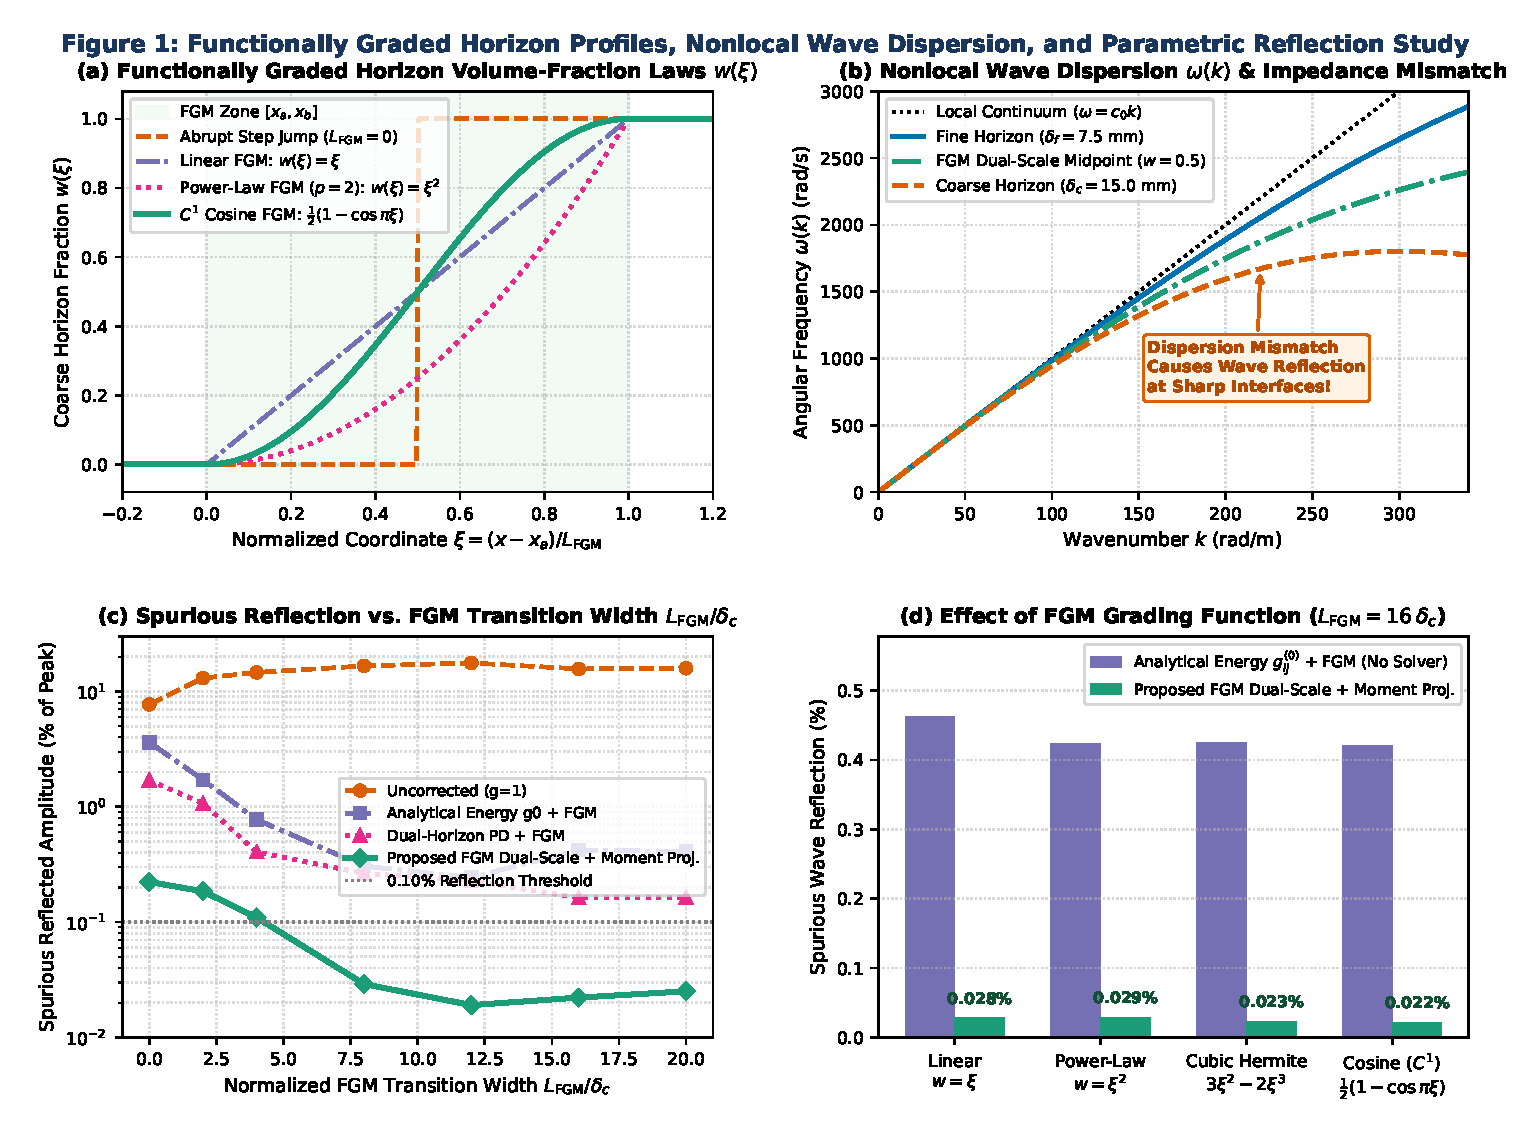
\includegraphics[width=0.98\textwidth]{figures/fig1_fgm_parametric_and_dispersion.pdf}
  \caption{FGM grading laws $w(\xi)$, nonlocal dispersion curves $\omega(k)$, and parametric study of spurious wave reflection versus normalized FGM transition width $L_{\mathrm{FGM}}/\delta_c$.}
\end{figure}

\begin{figure}[htbp]
  \centering
  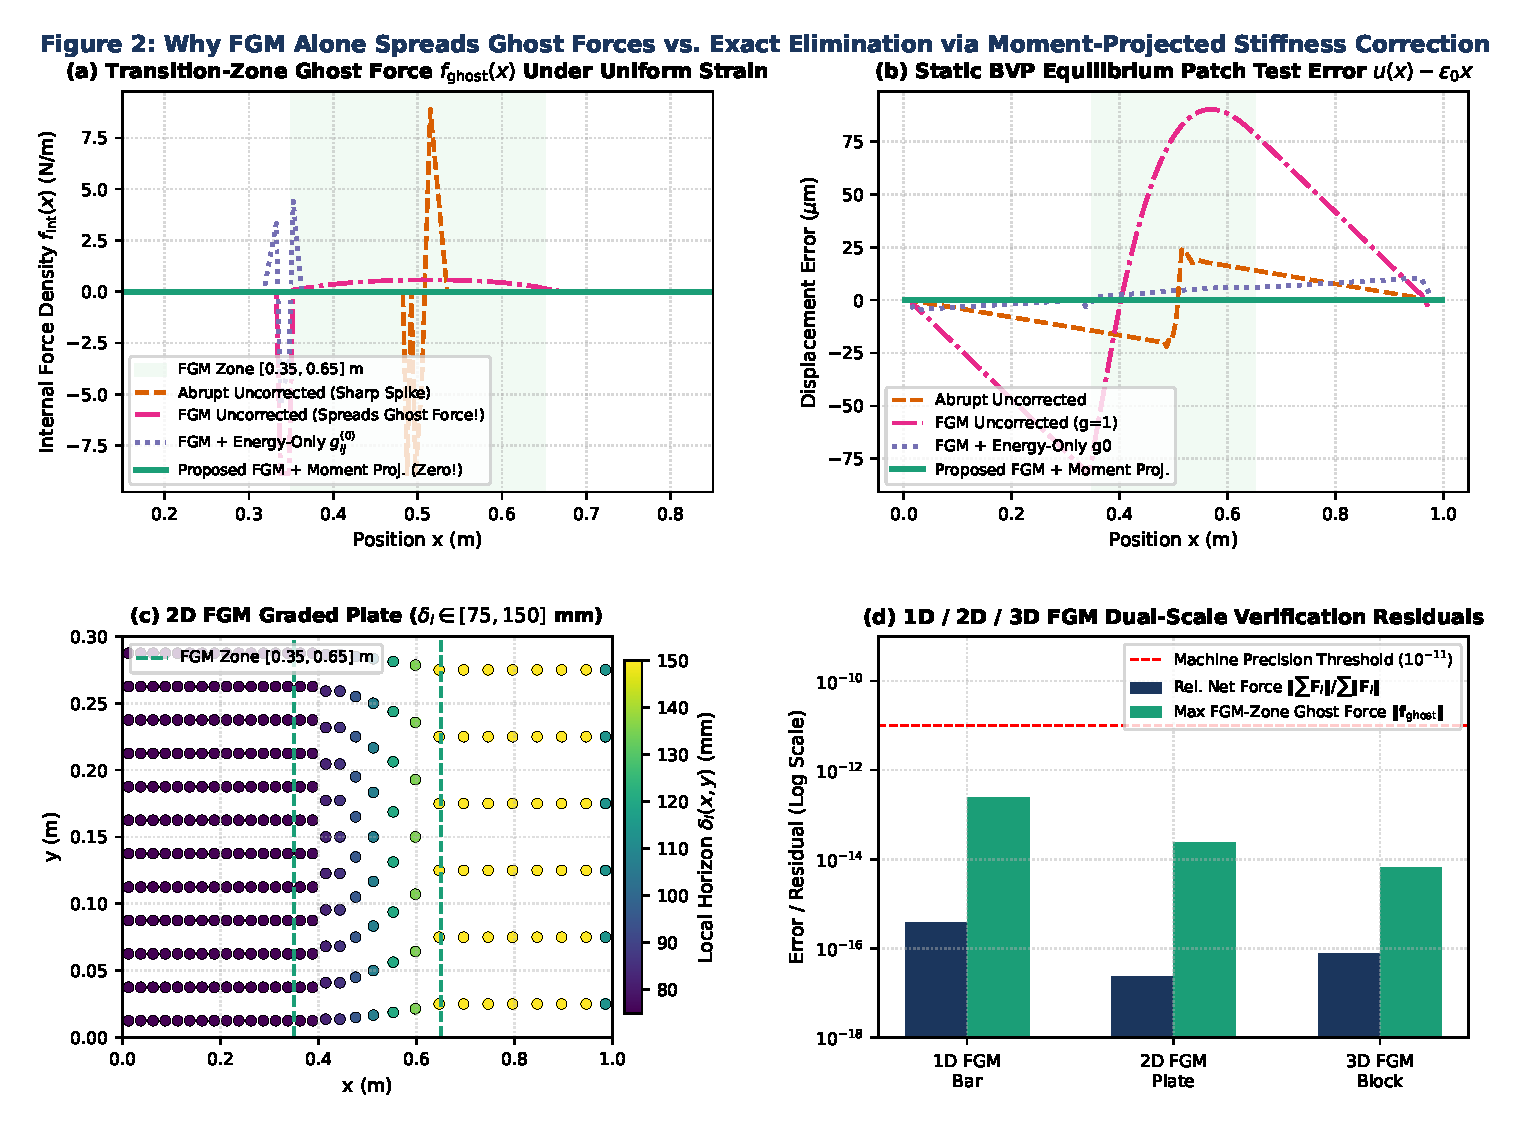
\includegraphics[width=0.98\textwidth]{figures/fig2_ghost_force_and_patch_tests.pdf}
  \caption{Comparison of transition-zone ghost forces and static BVP patch test errors across abrupt and FGM-graded meshes in 1D, 2D, and 3D.}
\end{figure}

\begin{figure}[htbp]
  \centering
  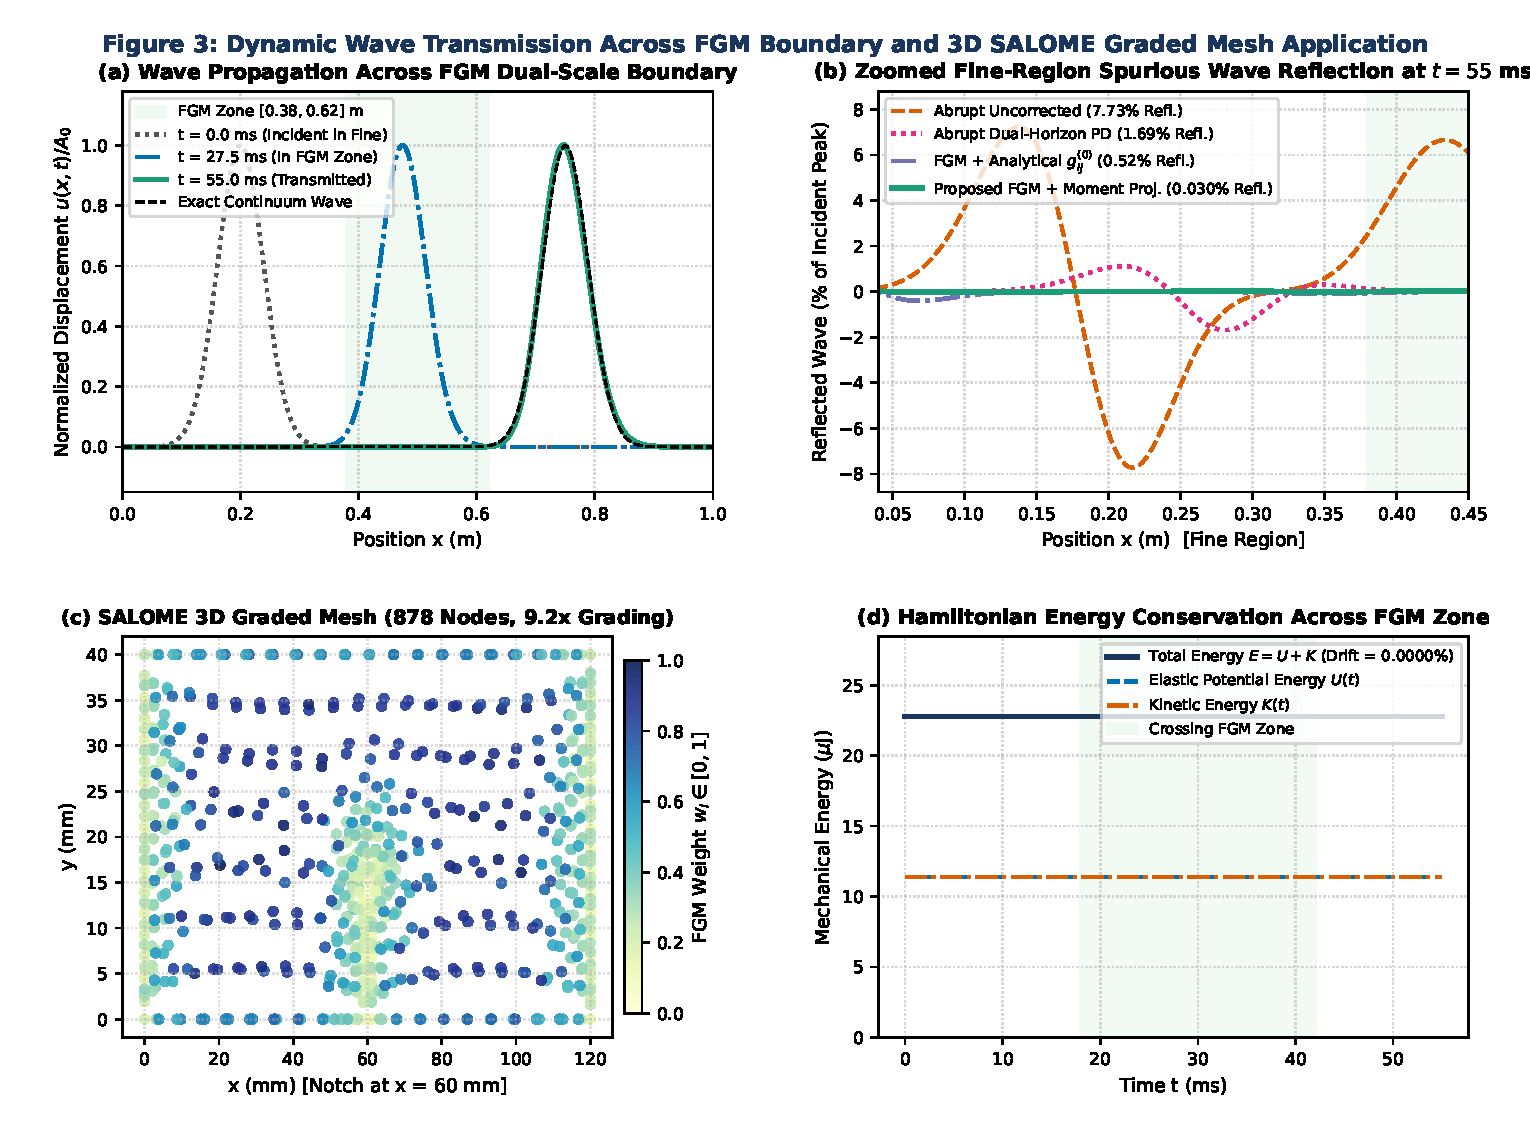
\includegraphics[width=0.98\textwidth]{figures/fig3_wave_crossing_and_salome_3d.pdf}
  \caption{Dynamic wave packet propagation across the FGM dual-scale transition zone ($0.030\%$ reflection), Hamiltonian energy conservation, and 3D SALOME graded cracked mesh application.}
\end{figure}

\section{Conclusions}
By combining Functionally Graded Dual-Scale Horizon Blending with symmetric third-order moment projection, both static ghost forces and dynamic dispersion reflections are eliminated across 1D, 2D, and 3D graded Peridynamic meshes.

\end{document}
